\documentclass[11pt,a4paper]{article}
\usepackage[margin=2.3cm]{geometry}
\usepackage{amsmath,booktabs,graphicx,float}
\usepackage[hidelinks]{hyperref}
\graphicspath{{figures/}}
\title{Singapore Rainfall: Patterns and 30-Minute Exceedance Forecasting}
\author{Group members and student IDs: \textit{to be completed}}
\date{}
\begin{document}
\maketitle
\section{Data, cleaning and computing environment}
We use NEA rainfall observations from 2017 through 2024. The original fields include observation timestamp, station ID, station metadata, coordinates and five-minute rainfall totals in millimetres. The official collection states that timestamps use Singapore Time and that records may be missing and have not undergone climate-data quality control.

Data source: \url{https://data.gov.sg/collections/2279/view}.
All processing uses Spark DataFrames. Exact semantic duplicates are removed. Conflicting observations at the same station and timestamp are excluded. Negative, nonfinite, unparseable, geographically invalid and off-grid observations are excluded. Early timestamps within one second of the five-minute grid are aligned and audited. Missing observations are never treated as zero rainfall. Five-minute values above 50 mm are retained and flagged as an engineering audit rule, not an official weather limit.

\begin{table}[H]\centering\small
\caption{Record-level quality audit; off-grid counts include accepted one-second alignment.}
\resizebox{\textwidth}{!}{\begin{tabular}{llllll}
\toprule
Year & Raw & Invalid & Off-grid & Unique valid & Clean \\
\midrule
2017 & 5256106 & 0 & 1775327 & 5256022 & 5256018 \\
2018 & 4594246 & 0 & 0 & 4594246 & 4594246 \\
2019 & 5026862 & 0 & 0 & 5026862 & 5026862 \\
2020 & 6334473 & 0 & 0 & 6334473 & 6334473 \\
2021 & 7044646 & 0 & 0 & 7044646 & 7044646 \\
2022 & 7133230 & 0 & 0 & 7133230 & 7133230 \\
2023 & 6742890 & 0 & 0 & 6742890 & 6742890 \\
2024 & 6406260 & 0 & 0 & 6406260 & 6406260 \\
\bottomrule\end{tabular}}
\end{table}
1 stations have more than one distinct coordinate pair. These changes can represent metadata updates or relocation; fixed IDs do not guarantee fixed physical locations.

\begin{table}[H]\centering\small
\caption{Local Spark runtime configuration}
\resizebox{\textwidth}{!}{\begin{tabular}{ll}
\toprule
Setting & Value \\
\midrule
spark & 3.5.3 \\
logical\_cpus & 10 \\
ram\_bytes & 10428227584 \\
master & local[6] \\
shuffle\_partitions & 16 \\
java & 11.0.13 \\
driver\_memory & 4g \\
\bottomrule\end{tabular}}
\end{table}
Python: 3.12.3 (main, Aug 31 2026, 10:18:26) [GCC 13.3.0]. Platform: Linux-6.18.33.1-microsoft-standard-WSL2-x86\_64-with-glibc2.39.

\begin{table}[H]\centering\small
\caption{Measured stage elapsed times; preparation includes cleaning and exploratory aggregation.}
\resizebox{\textwidth}{!}{\begin{tabular}{ll}
\toprule
Stage & Seconds \\
\midrule
prepare & 653.6 \\
train & 1517.2 \\
\bottomrule\end{tabular}}
\end{table}
\section{Exploratory analysis}
A station-day is used for daily statistics only when at least 95\% of its 288 expected intervals are observed. Monthly statistics report numbers of qualifying station-days. Annual sums cover qualifying days and are not complete climatological annual totals. Mean rainfall per valid day, wet-day frequency and positive-interval intensity are analysed separately to distinguish exposure, frequency and intensity.

Wet intervals and wet days here mean positive observed rainfall. This operational definition differs from the MSS climate rainday criterion of at least 0.2 mm; their counts are not directly comparable.

A common-ID panel contains 37 stations with qualifying days in every year. This controls changing station IDs, but annual valid-day counts and potential relocation must still be considered.

No station reaches 95\% full-year coverage in all eight years. The additional strict-coverage panel is therefore empty. The common-ID comparison does not eliminate missing-day bias.

Across qualifying station-days, month 11 has the highest mean daily rainfall (10.54 mm) and month 7 the lowest (5.05 mm). These means are weighted by qualifying station-day counts.

The maximum month/hour wet-interval fraction is 0.104, occurring in month 11 at hour 15 SGT.

MSS long-term climatology describes wetter conditions in November-January and more frequent afternoon rainfall, with February as the driest month. Differences from this study can reflect different periods, station mixtures and completeness filtering; their contributions cannot be identified from these data alone.

Climate context: \url{https://www.weather.gov.sg/climate-climate-of-singapore/}.
\begin{table}[H]\centering\small
\caption{Largest qualifying station-day totals, requiring further quality checks}
\resizebox{\textwidth}{!}{\begin{tabular}{llll}
\toprule
Station & Date & Observed daily mm & Coverage \\
\midrule
S107 & 2022-08-21 & 786.6 & 0.983 \\
S36 & 2021-04-01 & 319.60000999999994 & 1.000 \\
S107 & 2022-08-20 & 262.0 & 0.993 \\
S40 & 2021-08-24 & 247.19996999999995 & 1.000 \\
S205 & 2023-02-28 & 210.32400000000004 & 1.000 \\
S24 & 2021-01-10 & 205.4 & 1.000 \\
S224 & 2021-01-10 & 197.784 & 1.000 \\
S208 & 2021-01-10 & 197.06400000000005 & 1.000 \\
S61 & 2023-02-28 & 196.39999999999998 & 1.000 \\
S113 & 2023-02-28 & 194.20000000000005 & 1.000 \\
\bottomrule\end{tabular}}
\end{table}
These are observed, unvalidated extremes. In particular, very large daily totals require cross-station and provider checks before being treated as physical weather records. No positive outlier was silently removed.

\begin{table}[H]\centering\small
\caption{Positive-value audit; absence of a flag does not establish climate-data validity}
\resizebox{\textwidth}{!}{\begin{tabular}{lll}
\toprule
Year & Flagged intervals & Maximum five-minute mm \\
\midrule
2017 & 0 & 18.0 \\
2018 & 0 & 15.6 \\
2019 & 0 & 15.4 \\
2020 & 0 & 20.6 \\
2021 & 0 & 26.4 \\
2022 & 0 & 37.2 \\
2023 & 0 & 17.622 \\
2024 & 0 & 15.912 \\
\bottomrule\end{tabular}}
\end{table}
\section{Prediction protocol}
The external interface accepts station ID, prediction time and rainfall threshold. The program retrieves observations through the prediction time internally. Predictions are retrospective: the latest reading is assumed already available. Historical update timestamps can lag observation times, so this experiment does not establish real-time publication latency.

\[R_{30}(s,t)=\sum_{k=1}^{6}r(s,t+5k\text{ minutes}),\qquad y(s,t,a)=\mathbf{1}[R_{30}(s,t)>a].\]
The original reading type confirms a five-minute total, but the official collection does not establish whether its timestamp is the start or end of the accumulation interval. The target therefore represents the next six recorded observations; physical interval-end semantics remain an assumption.

Training uses 2017-2021, validation uses 2022 and testing uses 2023-2024. Targets crossing split boundaries are excluded. Complete examples require 12 past readings at t-55 through t and six future readings at t+5 through t+30. No future observations enter features. Encoders, standardisation and baseline probabilities are fitted using training data only.

Training uses prediction origins every 30 minutes and a uniform origin fraction of 0.100. The stable station/time hash uses seed 42. All four threshold examples from a retained origin remain together. Validation and main testing retain all complete 30-minute origins; an additional evaluation retains all complete five-minute test origins. No class-dependent sampling or reweighting is used.

There are 48,538,625 cleaned readings and 47,048,853 complete windows. The fraction excluded by window completeness is 3.07 percent.

\begin{table}[H]\centering\small
\caption{Main experiment sample counts after completeness, temporal boundaries and training sampling}
\resizebox{\textwidth}{!}{\begin{tabular}{ll}
\toprule
Split & Threshold-expanded examples \\
\midrule
train & 1,796,204 \\
validation & 4,714,860 \\
test & 8,683,544 \\
\bottomrule\end{tabular}}
\end{table}
\begin{table}[H]\centering\small
\caption{Feature groups; all history ends at prediction time}
\resizebox{\textwidth}{!}{\begin{tabular}{ll}
\toprule
Features & Contents \\
\midrule
F0 & Station encoding, coordinates, cyclical hour/day-of-year, threshold \\
F1 & F0 plus current five-minute rainfall and six five-minute lags \\
F2 & F1 plus 15/30/60-minute sums, 60-minute maximum, wet count and 15-minute trend \\
\bottomrule\end{tabular}}
\end{table}
Thresholds are 0, 1, 5 and 10 mm, using strict exceedance. A single joint binary classifier includes threshold as a numeric feature. Other nonnegative thresholds can be queried but are not independently validated. Thresholds are experimental settings, not official warning levels.

Models are MLlib logistic regression, random forest and gradient-boosted trees. LR regularisation is 0.01/0.1/1; RF uses 50/100 trees at depth 5/8; GBT uses 30/60 iterations at depth 3/5. Identical fitted F2 preprocessing is shared across candidates. Hyperparameters are selected by validation macro Brier score, averaging the four thresholds equally. The winner family and parameters are frozen for the F0/F1/F2 ablation. We do not use random cross-validation or test results for tuning.

B0 predicts training exceedance frequency by threshold. B1 uses training station/month/threshold frequency, falling back to B0 for absent cells. Probability evaluation reports Brier score, log loss, Spark PR-AUC and ROC-AUC. AUC is unavailable in single-class subsets. Reliability plots use ten equal-width probability bins. Per-threshold decision cutoffs maximise validation F1 over 0.05 to 0.95, then remain fixed for test classification metrics.

MLlib source: \url{https://spark.apache.org/docs/3.5.3/ml-classification-regression.html}.
\section{Predictive results}
\begin{table}[H]\centering\small
\caption{Chronological validation model selection; lower Brier is better}
\resizebox{\textwidth}{!}{\begin{tabular}{lll}
\toprule
Model & Parameters & Validation macro Brier \\
\midrule
lr & \{'regParam': 0.01\} & 0.01871 \\
lr & \{'regParam': 0.1\} & 0.02097 \\
lr & \{'regParam': 1.0\} & 0.02327 \\
rf & \{'numTrees': 50, 'maxDepth': 5\} & 0.01752 \\
rf & \{'numTrees': 50, 'maxDepth': 8\} & 0.01609 \\
rf & \{'numTrees': 100, 'maxDepth': 5\} & 0.01774 \\
rf & \{'numTrees': 100, 'maxDepth': 8\} & 0.01632 \\
gbt & \{'maxIter': 30, 'maxDepth': 3\} & 0.01561 \\
gbt & \{'maxIter': 30, 'maxDepth': 5\} & 0.01533 \\
gbt & \{'maxIter': 60, 'maxDepth': 3\} & 0.01493 \\
gbt & \{'maxIter': 60, 'maxDepth': 5\} & 0.01474 \\
\bottomrule\end{tabular}}
\end{table}
Selected model: gbt, parameters \{'maxIter': 60, 'maxDepth': 5\}.

\subsection{B0 baseline}
\begin{table}[H]\centering\small
\caption{B0 baseline}
\resizebox{\textwidth}{!}{\begin{tabular}{lllllll}
\toprule
mm & N & Positive fraction & Brier & PR-AUC & ROC-AUC & Log loss \\
\midrule
0.0 & 2,170,886 & 0.06527 & 0.06105 & 0.06527 & 0.50000 & 0.24158 \\
1.0 & 2,170,886 & 0.02604 & 0.02537 & 0.02604 & 0.50000 & 0.12095 \\
5.0 & 2,170,886 & 0.00857 & 0.00850 & 0.00857 & 0.50000 & 0.04934 \\
10.0 & 2,170,886 & 0.00399 & 0.00397 & 0.00399 & 0.50000 & 0.02602 \\
\bottomrule\end{tabular}}
\end{table}
Macro Brier score: 0.02472.

\subsection{B1 seasonal baseline}
\begin{table}[H]\centering\small
\caption{B1 seasonal baseline}
\resizebox{\textwidth}{!}{\begin{tabular}{lllllll}
\toprule
mm & N & Positive fraction & Brier & PR-AUC & ROC-AUC & Log loss \\
\midrule
0.0 & 2,170,886 & 0.06527 & 0.06109 & 0.07958 & 0.55094 & 0.25965 \\
1.0 & 2,170,886 & 0.02604 & 0.02545 & 0.02960 & 0.52843 & 0.13921 \\
5.0 & 2,170,886 & 0.00857 & 0.00853 & 0.00874 & 0.50609 & 0.06951 \\
10.0 & 2,170,886 & 0.00399 & 0.00399 & 0.00402 & 0.50333 & 0.04991 \\
\bottomrule\end{tabular}}
\end{table}
Macro Brier score: 0.02476.

\subsection{Selected model, 30-minute origins}
\begin{table}[H]\centering\small
\caption{Selected model, 30-minute origins}
\resizebox{\textwidth}{!}{\begin{tabular}{lllllll}
\toprule
mm & N & Positive fraction & Brier & PR-AUC & ROC-AUC & Log loss \\
\midrule
0.0 & 2,170,886 & 0.06527 & 0.03283 & 0.67985 & 0.88764 & 0.13506 \\
1.0 & 2,170,886 & 0.02604 & 0.01543 & 0.58686 & 0.85551 & 0.07397 \\
5.0 & 2,170,886 & 0.00857 & 0.00658 & 0.37619 & 0.88655 & 0.04189 \\
10.0 & 2,170,886 & 0.00399 & 0.00359 & 0.25024 & 0.88661 & 0.03093 \\
\bottomrule\end{tabular}}
\end{table}
Macro Brier score: 0.01461.

\subsection{Selected model, five-minute origins}
\begin{table}[H]\centering\small
\caption{Selected model, five-minute origins}
\resizebox{\textwidth}{!}{\begin{tabular}{lllllll}
\toprule
mm & N & Positive fraction & Brier & PR-AUC & ROC-AUC & Log loss \\
\midrule
0.0 & 13,025,429 & 0.06520 & 0.03283 & 0.68585 & 0.88090 & 0.13506 \\
1.0 & 13,025,429 & 0.02601 & 0.01539 & 0.58234 & 0.87656 & 0.07386 \\
5.0 & 13,025,429 & 0.00856 & 0.00658 & 0.37298 & 0.84395 & 0.04190 \\
10.0 & 13,025,429 & 0.00398 & 0.00359 & 0.24719 & 0.85578 & 0.03093 \\
\bottomrule\end{tabular}}
\end{table}
Macro Brier score: 0.01460.

The selected model changes macro Brier by -40.92 percent relative to B0 on main test origins (negative denotes improvement). Per-threshold results must also be considered, particularly when exceedance is rare.

\begin{table}[H]\centering\small
\caption{Feature ablation with frozen winner family and hyperparameters}
\resizebox{\textwidth}{!}{\begin{tabular}{lll}
\toprule
Feature group & Validation macro Brier & Test macro Brier \\
\midrule
F0 & 0.02461 & 0.02441 \\
F1 & 0.01490 & 0.01480 \\
F2 & 0.01474 & 0.01461 \\
\bottomrule\end{tabular}}
\end{table}
Adding current rainfall and recent lags changes held-out macro Brier from 0.02441 (F0) to 0.01480 (F1). Adding rolling summaries changes it to 0.01461 (F2). These frozen-parameter comparisons quantify the incremental predictive value of recent observations and their summaries.

\begin{table}[H]\centering\small
\caption{Main test classification at validation-selected operating points}
\resizebox{\textwidth}{!}{\begin{tabular}{lllll}
\toprule
Rain mm & Probability cutoff & Precision & Recall & F1 \\
\midrule
0.0 & 0.3 & 0.69769 & 0.60124 & 0.64589 \\
1.0 & 0.25 & 0.65060 & 0.53531 & 0.58735 \\
5.0 & 0.2 & 0.44779 & 0.47188 & 0.45952 \\
10.0 & 0.2 & 0.37298 & 0.39951 & 0.38579 \\
\bottomrule\end{tabular}}
\end{table}
30-minute origins: fraction of station/time examples with increasing probability as the rainfall threshold rises = 0.00010. Monotonicity is measured, not enforced.

Five-minute origins: fraction of station/time examples with increasing probability as the rainfall threshold rises = 0.00010. Monotonicity is measured, not enforced.

\begin{table}[H]\centering\small
\caption{Test subgroup probability performance}
\resizebox{\textwidth}{!}{\begin{tabular}{lllll}
\toprule
Year & Rain mm & N & Positive fraction & Brier \\
\midrule
2023 & 0.0 & 1114386 & 0.06680 & 0.03306 \\
2023 & 1.0 & 1114386 & 0.02630 & 0.01558 \\
2023 & 5.0 & 1114386 & 0.00876 & 0.00670 \\
2023 & 10.0 & 1114386 & 0.00414 & 0.00372 \\
2024 & 0.0 & 1056500 & 0.06365 & 0.03259 \\
2024 & 1.0 & 1056500 & 0.02576 & 0.01526 \\
2024 & 5.0 & 1056500 & 0.00837 & 0.00645 \\
2024 & 10.0 & 1056500 & 0.00383 & 0.00345 \\
\bottomrule\end{tabular}}
\end{table}
\begin{table}[H]\centering\small
\caption{Test subgroup probability performance}
\resizebox{\textwidth}{!}{\begin{tabular}{lllll}
\toprule
Currently wet (0/1) & Rain mm & N & Positive fraction & Brier \\
\midrule
0 & 0.0 & 2102846 & 0.03967 & 0.03074 \\
0 & 1.0 & 2102846 & 0.01056 & 0.01036 \\
0 & 5.0 & 2102846 & 0.00327 & 0.00353 \\
0 & 10.0 & 2102846 & 0.00136 & 0.00168 \\
1 & 0.0 & 68040 & 0.85641 & 0.09748 \\
1 & 1.0 & 68040 & 0.50454 & 0.17201 \\
1 & 5.0 & 68040 & 0.17225 & 0.10085 \\
1 & 10.0 & 68040 & 0.08511 & 0.06247 \\
\bottomrule\end{tabular}}
\end{table}
Additional month and station subgroup tables are exported as CSV. Differences in Brier across subgroups can reflect both forecast errors and different event prevalence; they should not be read as a pure ranking of station difficulty. Adjacent time windows and stations are dependent, so no independent-sample confidence intervals are claimed.

Model reload validation: 20 probe examples have matching saved/reloaded probabilities within 1e-12 (passed: True). Automated tests separately check exact windows, strict exceedance, missing future records, future-feature leakage, temporal boundaries, timestamp alignment and single-class metrics.

\section{Figures}
\begin{figure}[htbp]\centering
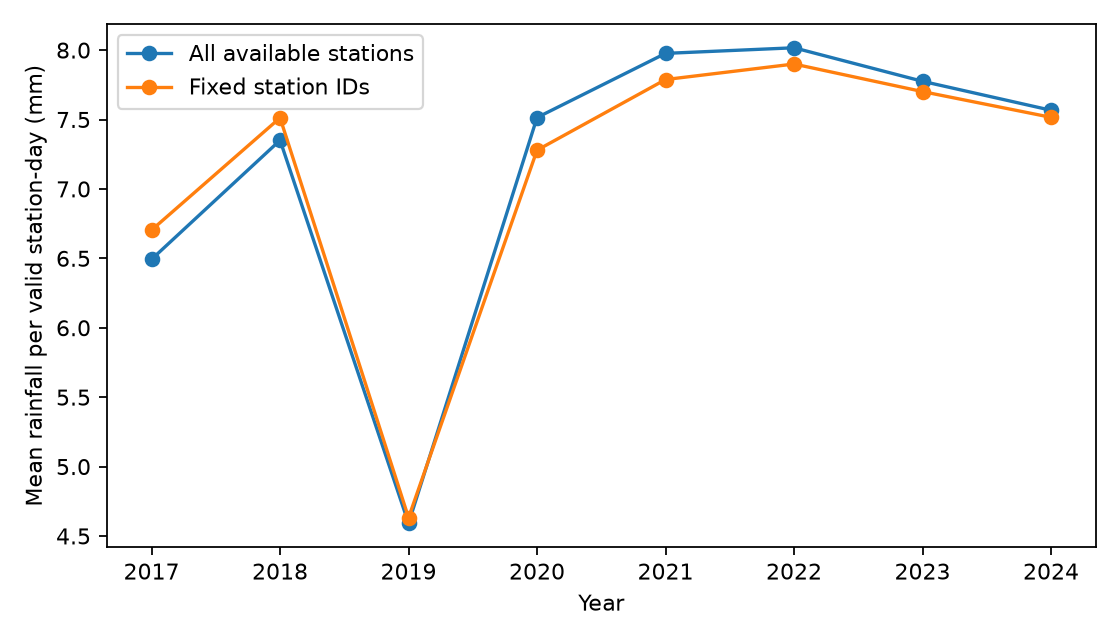
\includegraphics[width=0.95\textwidth,height=0.65\textheight,keepaspectratio]{annual_daily_mean.png}
\caption{Rainfall per valid station-day for all available stations and common station IDs.}
\end{figure}
\begin{figure}[htbp]\centering
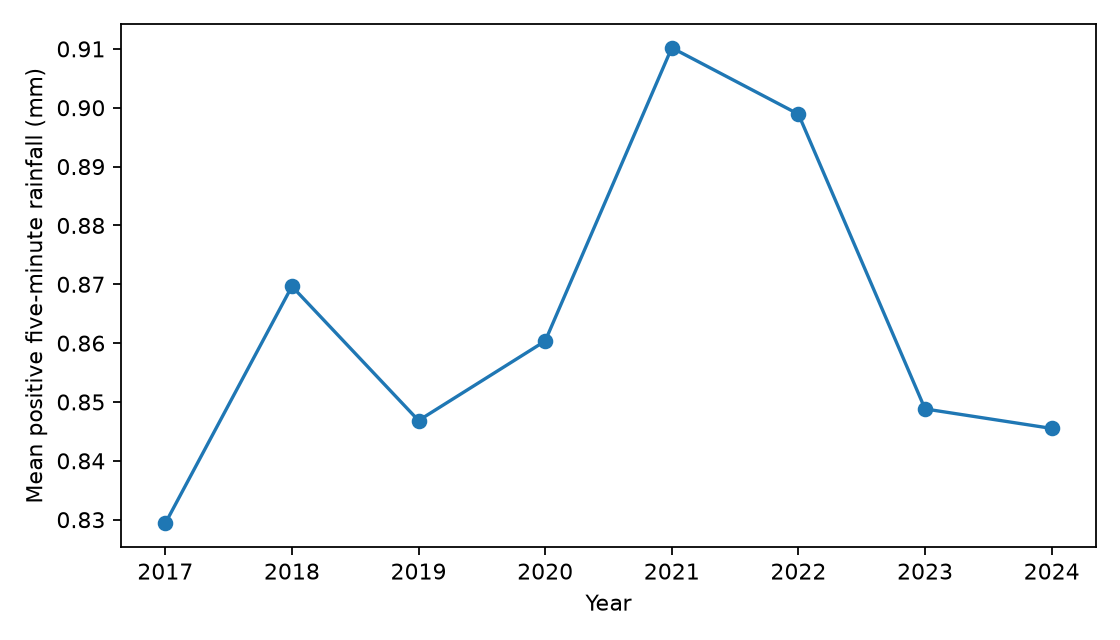
\includegraphics[width=0.95\textwidth,height=0.65\textheight,keepaspectratio]{annual_intensity.png}
\caption{Mean positive five-minute rainfall intensity.}
\end{figure}
\begin{figure}[htbp]\centering
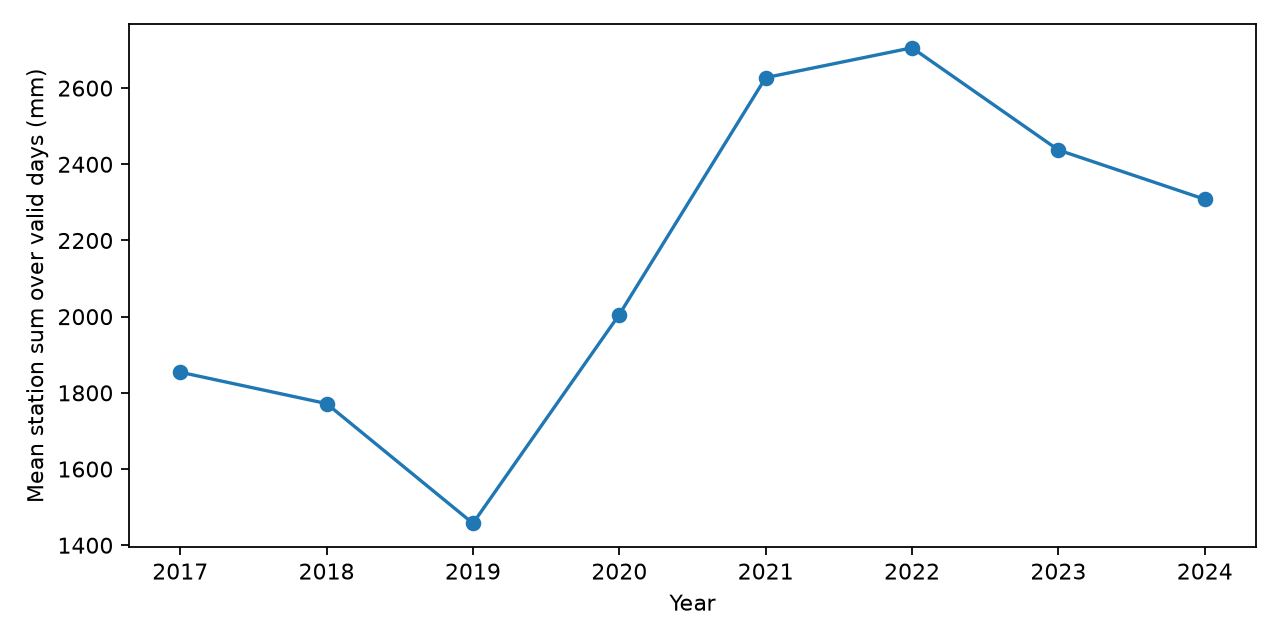
\includegraphics[width=0.95\textwidth,height=0.65\textheight,keepaspectratio]{annual_station.png}
\caption{Mean observed station cumulative rainfall over qualifying days; not complete annual climate totals.}
\end{figure}
\begin{figure}[htbp]\centering
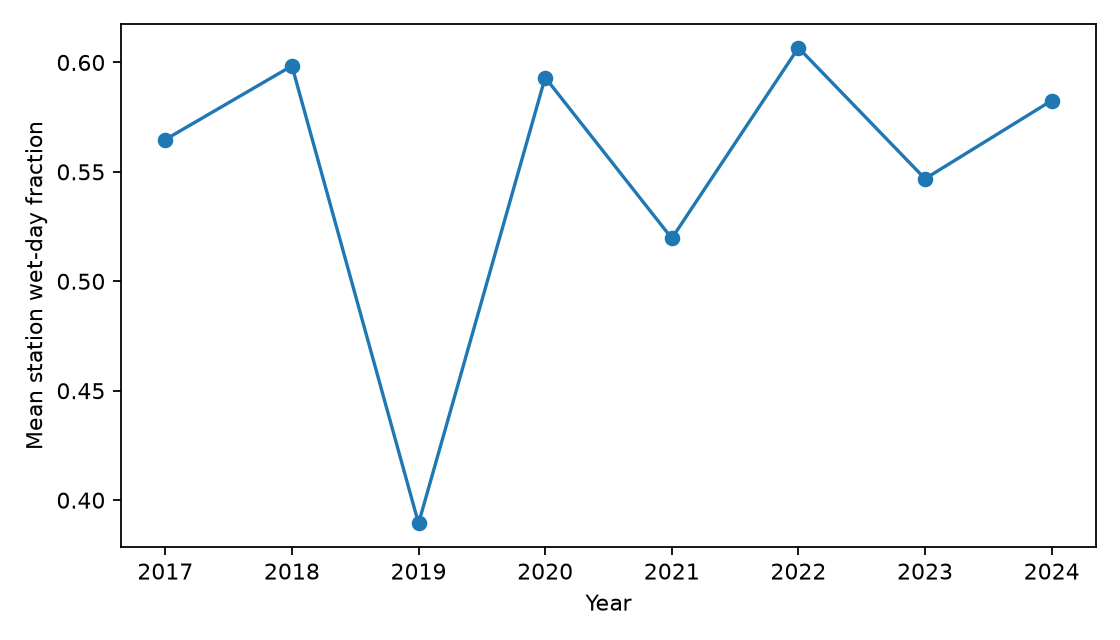
\includegraphics[width=0.95\textwidth,height=0.65\textheight,keepaspectratio]{annual_wet_days.png}
\caption{Mean station wet-day fraction among qualifying days.}
\end{figure}
\begin{figure}[htbp]\centering
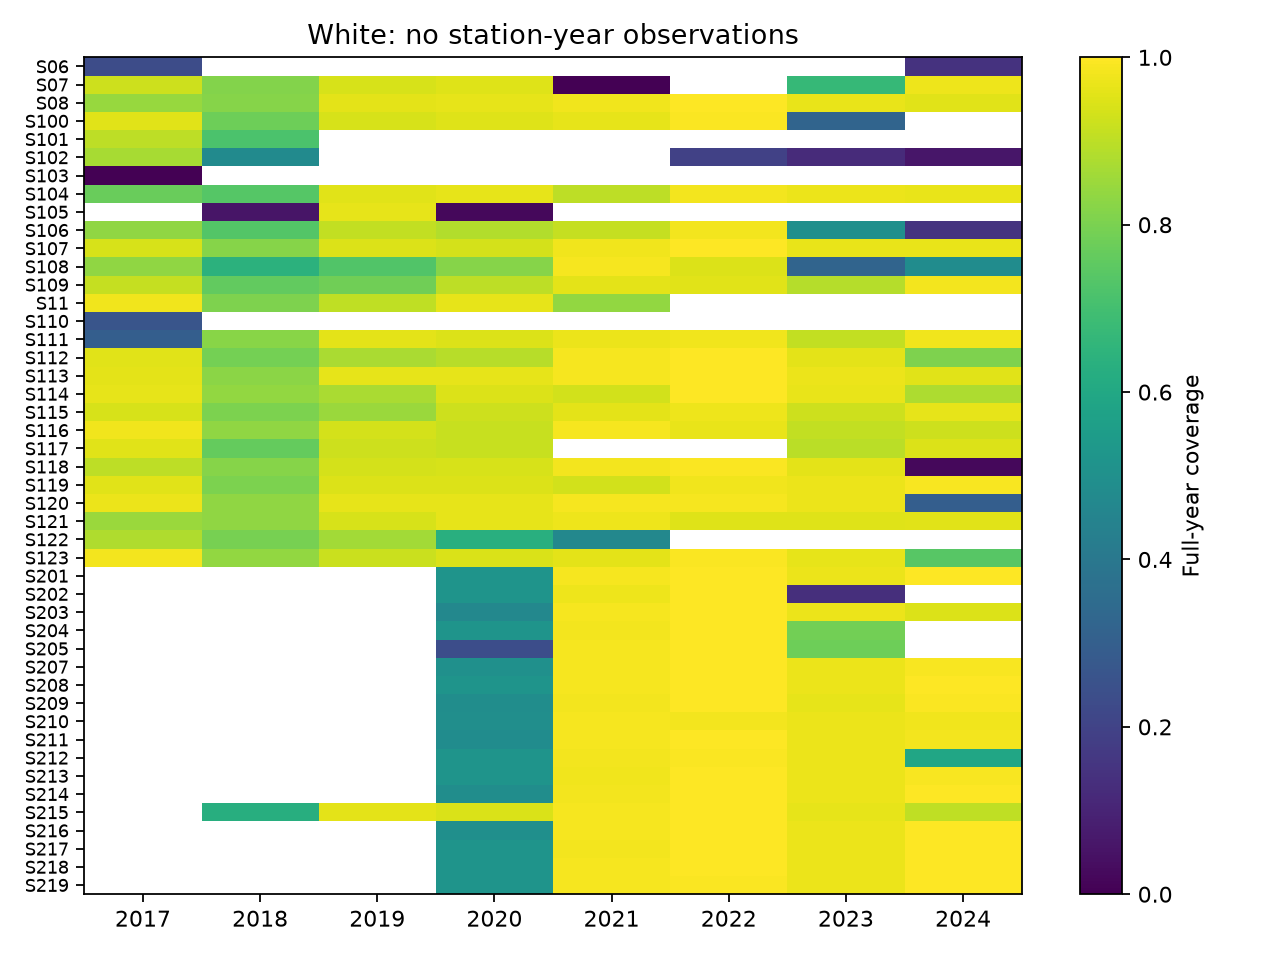
\includegraphics[width=0.95\textwidth,height=0.65\textheight,keepaspectratio]{coverage_part_1.png}
\caption{Full-year observation coverage, station panel 1; white cells have no observations.}
\end{figure}
\begin{figure}[htbp]\centering
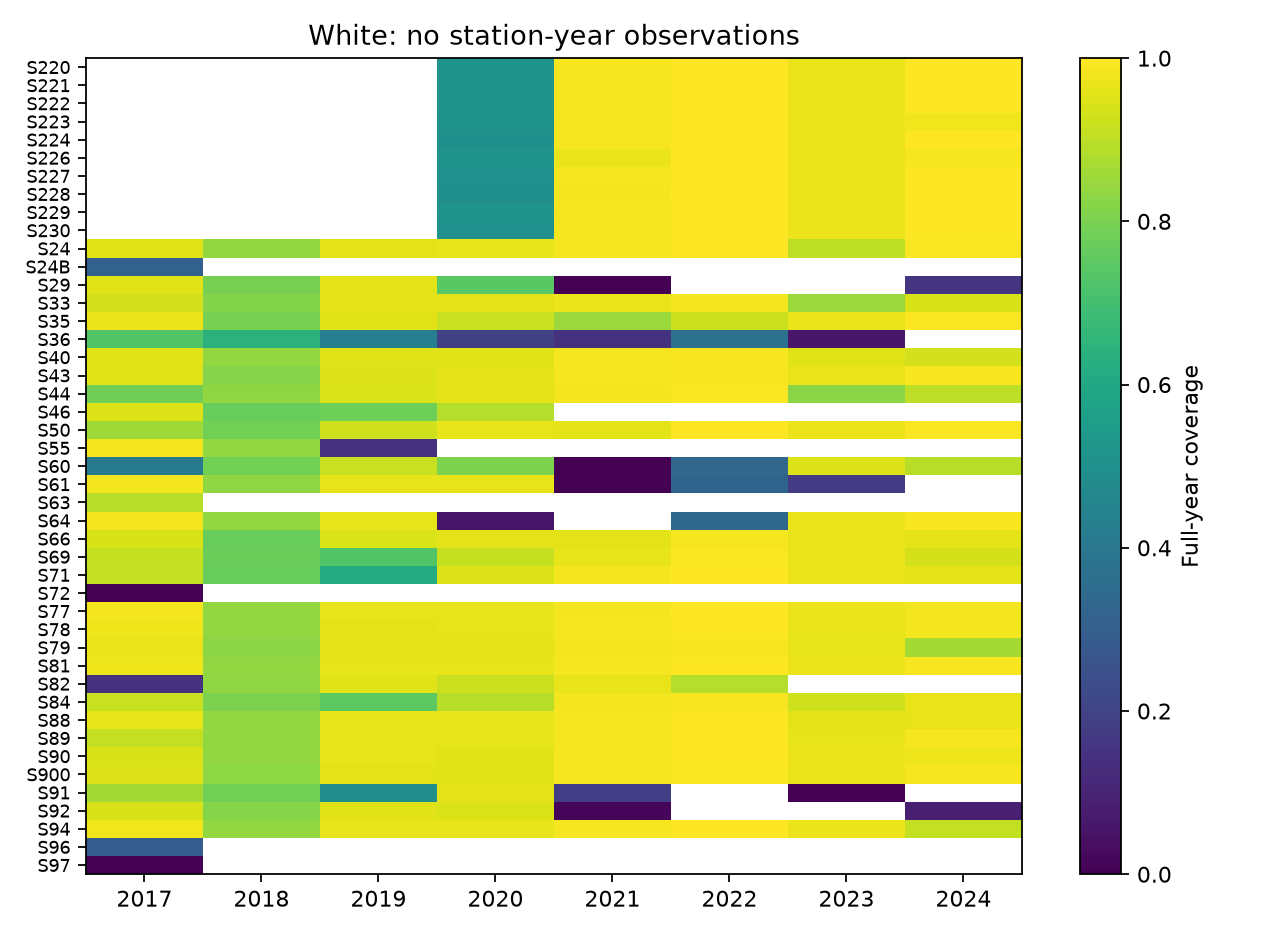
\includegraphics[width=0.95\textwidth,height=0.65\textheight,keepaspectratio]{coverage_part_2.png}
\caption{Full-year observation coverage, station panel 2; white cells have no observations.}
\end{figure}
\begin{figure}[htbp]\centering
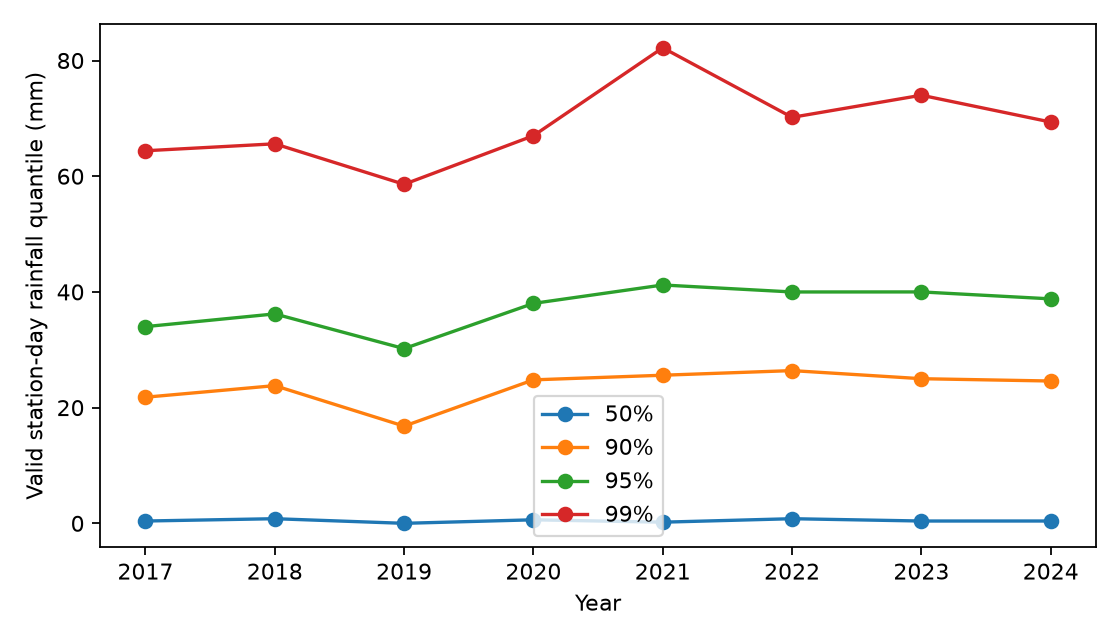
\includegraphics[width=0.95\textwidth,height=0.65\textheight,keepaspectratio]{daily_quantiles.png}
\caption{Quantiles of qualifying station-day rainfall.}
\end{figure}
\begin{figure}[htbp]\centering
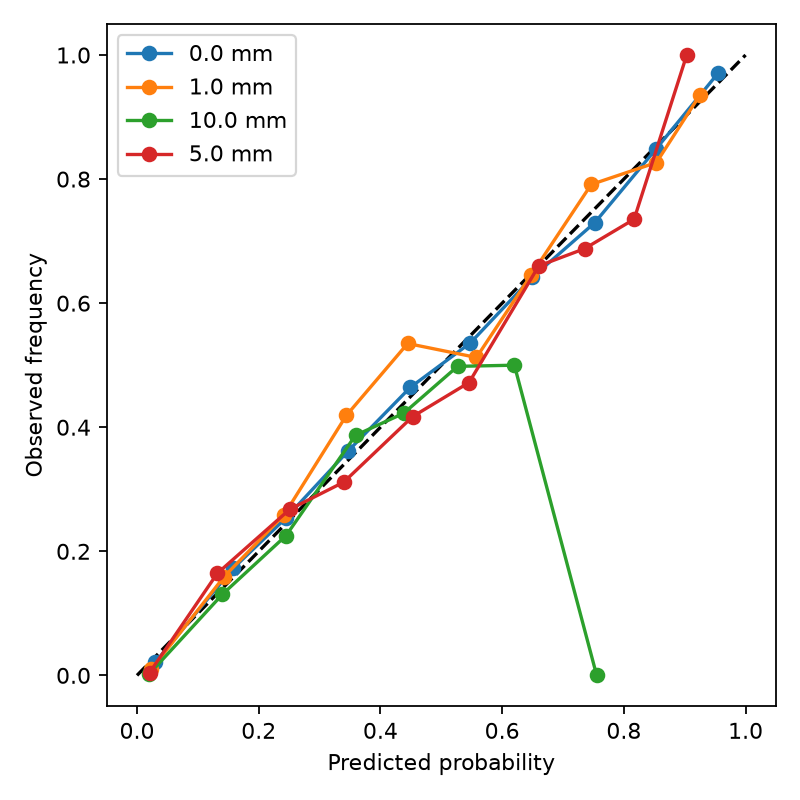
\includegraphics[width=0.95\textwidth,height=0.65\textheight,keepaspectratio]{five_minute_test_calibration.png}
\caption{Reliability at five-minute test origins.}
\end{figure}
\begin{figure}[htbp]\centering
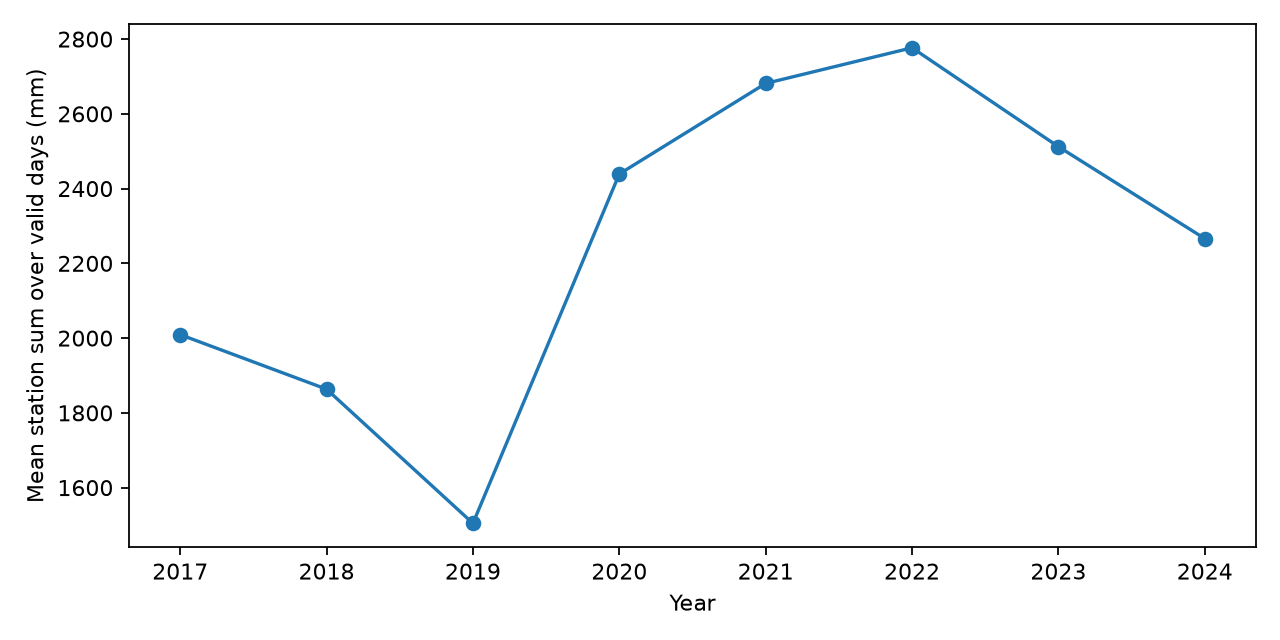
\includegraphics[width=0.95\textwidth,height=0.65\textheight,keepaspectratio]{fixed_station_annual.png}
\caption{Observed cumulative rainfall for the fixed-ID panel; remaining valid-day differences still matter.}
\end{figure}
\begin{figure}[htbp]\centering
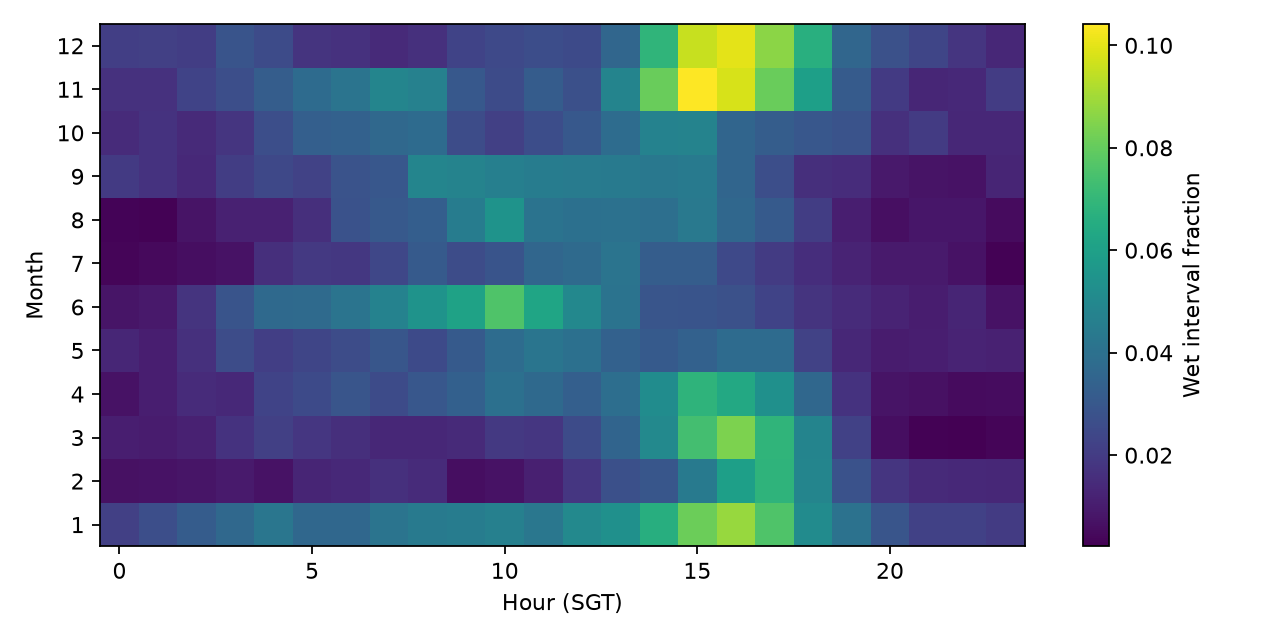
\includegraphics[width=0.95\textwidth,height=0.65\textheight,keepaspectratio]{month_hour.png}
\caption{Wet-interval frequency by month and local hour.}
\end{figure}
\begin{figure}[htbp]\centering
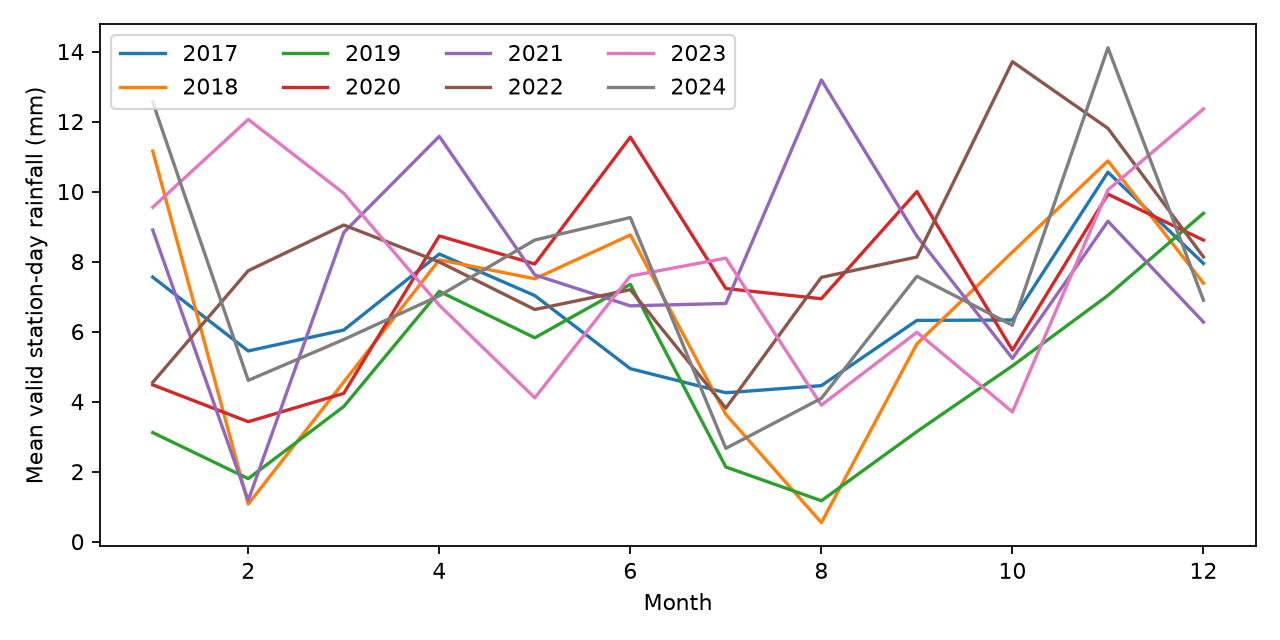
\includegraphics[width=0.95\textwidth,height=0.65\textheight,keepaspectratio]{monthly_rain.png}
\caption{Mean rainfall per qualifying station-day by year and month.}
\end{figure}
\begin{figure}[htbp]\centering
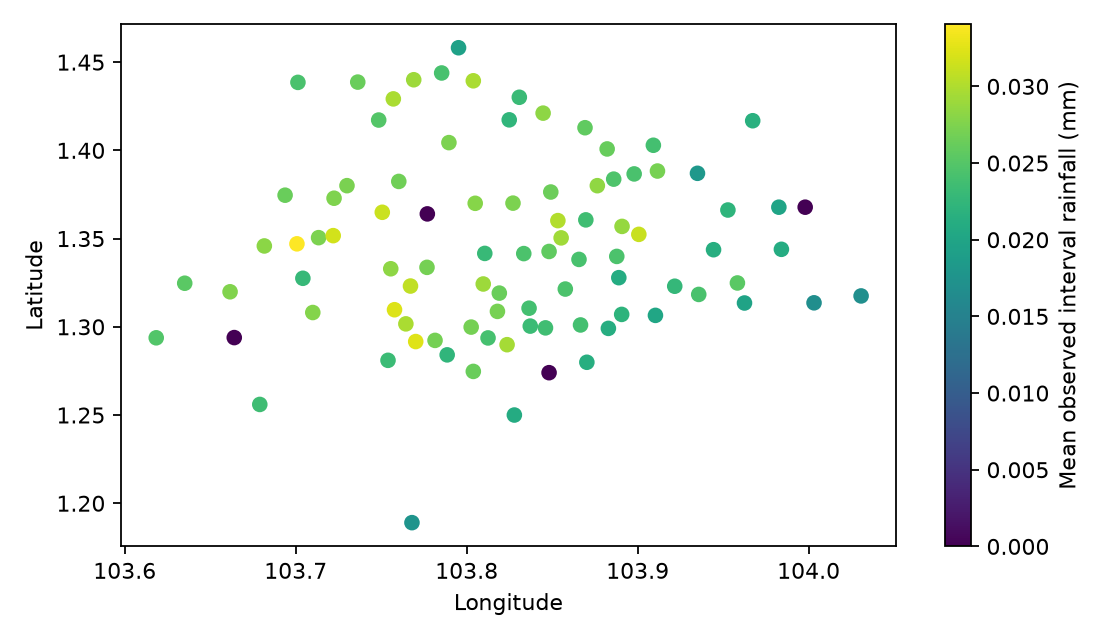
\includegraphics[width=0.95\textwidth,height=0.65\textheight,keepaspectratio]{stations.png}
\caption{Station coordinates coloured by mean observed five-minute rainfall; metadata changes may affect positions.}
\end{figure}
\begin{figure}[htbp]\centering
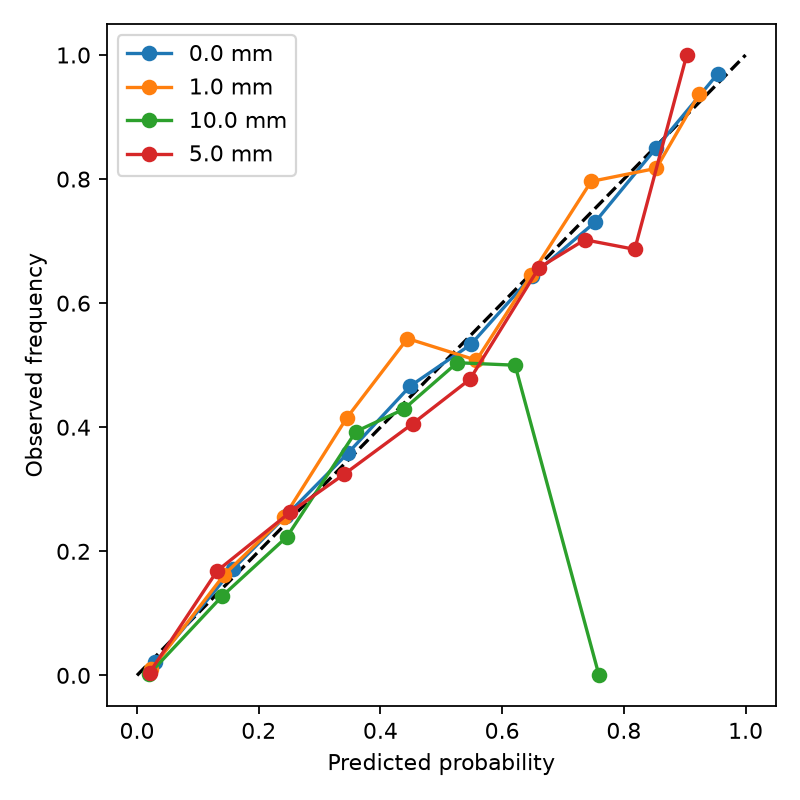
\includegraphics[width=0.95\textwidth,height=0.65\textheight,keepaspectratio]{test_calibration.png}
\caption{Reliability at 30-minute test origins; diagonal denotes perfect calibration.}
\end{figure}
\clearpage
\section{Limitations, further work and AI disclosure}
Eight years support descriptive comparisons, not proof of a long-term climate trend. Missingness and completeness filtering can bias both analysis and evaluation. Positive outliers have not received external quality control. Observed annual sums are incomplete when days fail coverage checks. A common station ID may have changing coordinates. Forecasts assume historical observations through t are available, and real-time data latency is not evaluated.

The models are assessed on the available network, not an independent unseen-station experiment. Outputs at other thresholds can be queried but are not separately validated; joint classifiers need not satisfy threshold monotonicity. Uniform training-origin sampling controls local computation but may lose rare training events. No radar, wind or neighbouring-station features are used. Further work could verify extreme events, test stable-location panels, improve calibration and enforce a coherent exceedance curve.

AI usage: OpenAI Codex assisted with experiment design, code implementation and LaTeX report generation. Group members should verify the implementation and actual results, complete member details and refine the interpretation before submission. Missing experiments are explicitly marked; no synthetic results are substituted for full-data experiments.

\end{document}
